
%(BEGIN_QUESTION)
% Copyright 2011, Tony R. Kuphaldt, released under the Creative Commons Attribution License (v 1.0)
% This means you may do almost anything with this work of mine, so long as you give me proper credit

The scrubber (vessel V-5) liquid level is being controlled by an Emerson DeltaV DCS, but something is wrong.  The operator reports seeing a liquid level of 90\% in the LG-31 sightglass while claiming the setpoint entered into the DeltaV Operate controller faceplate is 75\%:

$$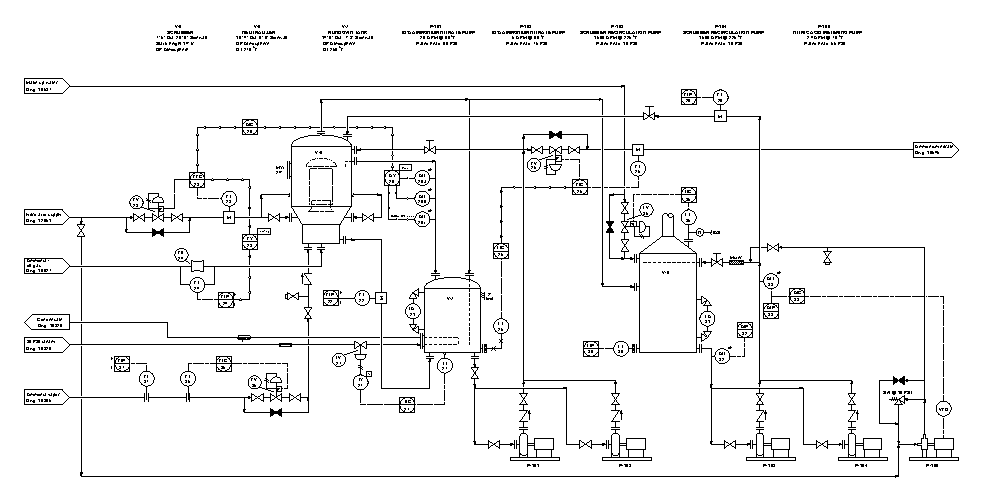
\includegraphics[width=15.5cm]{i0008rx01.eps}$$

\filbreak

A very useful feature of the {\it DeltaV Control Studio} application is being able to switch the view to ``online'' mode and watching real-time numerical data appear on the interconnecting lines between function blocks.  When you use the {\it Control Studio} software to examine this loop's function block program module in online mode, this is what you see:

$$\includegraphics[width=15.5cm]{i00961x02.eps}$$

Identify the likelihood of each specified fault in this process, based on what you see in the online Control Studio view.  Consider each fault one at a time (i.e. no coincidental faults), determining whether or not each fault could independently account for {\it all} measurements and symptoms in this process.

% No blank lines allowed between lines of an \halign structure!
% I use comments (%) instead, so that TeX doesn't choke.

$$\vbox{\offinterlineskip
\halign{\strut
\vrule \quad\hfil # \ \hfil & 
\vrule \quad\hfil # \ \hfil & 
\vrule \quad\hfil # \ \hfil \vrule \cr
\noalign{\hrule}
%
% First row
{\bf Fault} & {\bf Possible} & {\bf Impossible} \cr
%
\noalign{\hrule}
%
% Another row
Poor tuning in the PID function block &  &  \cr
%
\noalign{\hrule}
%
% Another row
LT-35 miscalibrated, reading too low &  &  \cr
%
\noalign{\hrule}
%
% Another row
LT-35 miscalibrated, reading too high &  &  \cr
%
\noalign{\hrule}
%
% Another row
Make-up water source shut off &  &  \cr
%
\noalign{\hrule}
%
% Another row
Pump P-103 failed (not pumping) &  &  \cr
%
\noalign{\hrule}
%
% Another row
LG-31 sightglass block valve plugged &  &  \cr
%
\noalign{\hrule}
%
% Another row
Pump P-105 failed (not pumping) &  &  \cr
%
\noalign{\hrule}
%
% Another row
Human operator error &  &  \cr
%
\noalign{\hrule}
} % End of \halign 
}$$ % End of \vbox


\underbar{file i00961}
%(END_QUESTION)





%(BEGIN_ANSWER)


%(END_ANSWER)





%(BEGIN_NOTES)

% No blank lines allowed between lines of an \halign structure!
% I use comments (%) instead, so that TeX doesn't choke.

$$\vbox{\offinterlineskip
\halign{\strut
\vrule \quad\hfil # \ \hfil & 
\vrule \quad\hfil # \ \hfil & 
\vrule \quad\hfil # \ \hfil \vrule \cr
\noalign{\hrule}
%
% First row
{\bf Fault} & {\bf Possible} & {\bf Impossible} \cr
%
\noalign{\hrule}
%
% Another row
Poor tuning in the PID function block &  & $\surd$ \cr
%
\noalign{\hrule}
%
% Another row
LT-35 miscalibrated, reading too low & $\surd$ &  \cr
%
\noalign{\hrule}
%
% Another row
LT-35 miscalibrated, reading too high &  & $\surd$ \cr
%
\noalign{\hrule}
%
% Another row
Make-up water source shut off &  & $\surd$ \cr
%
\noalign{\hrule}
%
% Another row
Pump P-103 failed (not pumping) &  & $\surd$ \cr
%
\noalign{\hrule}
%
% Another row
LG-31 sightglass block valve plugged & $\surd$ &  \cr
%
\noalign{\hrule}
%
% Another row
Pump P-105 failed (not pumping) &  & $\surd$ \cr
%
\noalign{\hrule}
%
% Another row
Human operator error & $\surd$ &  \cr
%
\noalign{\hrule}
} % End of \halign 
}$$ % End of \vbox


The high-saturated output of this level controller suggests a transmitter calibration error to be most likely.  While it is possible that the sightglass is reading (or was read) incorrectly, this alone would not explain why the controller output is so high.  However, since we do not know the typical operating position of LV-35, we cannot say with certainty that a position of 100\% necessary means trouble.  This also explains the potential for human operator error: it's possible that the operator mis-read the sightglass.











\filbreak \vskip 20pt \vbox{\hrule \hbox{\strut \vrule{} {\bf Virtual Troubleshooting} \vrule} \hrule}

\noindent
{\bf Predicting the effect of a given fault:} present each of the following faults to the students, one at a time, having them comment on all the effects each fault would produce.

\begin{itemize}
\item{} AIT-28c fails with a low ($<$ 4 mA) signal
\item{} FT-25 fails with a high ($>$ 20 mA) signal
\item{} VFD on P-105 miscalibrated so it spins 100 RPM slower than it's commanded to by AIC-33
\item{} AIC-28 set for incorrect action (direct/reverse)
\item{} TT-27 miscalibrated so it reads 7\% too low
\item{} FV-25 positioner miscalibrated so stem is 8\% more open than it should be
\item{} Bubbler tube (dip tube) on LT-35 plugs up ({\it INST240 review})
\item{} Field coils on FT-22 fail open ({\it INST241 review})
\item{} Field coils on FT-22 fail shorted ({\it INST241 review})
\item{} Capillary tube on LT-26 develops a leak ({\it INST240 review})
\item{} pH probe cable leading to input of AIT-32 fails shorted ({\it INST242 review})
\item{} Nozzle plugs in LV-35 positioner ({\it INST250 review})
\end{itemize}


\vskip 10pt


\noindent
{\bf Identifying possible/impossible faults:} present symptoms to the students and then have them determine whether or not a series of suggested faults could account for all the symptoms, explaining {\it why} or {\it why not} for each proposed fault:

\begin{itemize}
\item{} Symptom: {\it }
\item{}  -- {\bf Yes/No}
\item{}  -- {\bf Yes/No}
\item{}  -- {\bf Yes/No}
\end{itemize}


\vskip 10pt


\noindent
{\bf Determining the utility of given diagnostic tests:} present symptoms to the students and then propose the following diagnostic tests one by one.  Students rate the value of each test, determining whether or not it would give useful information (i.e. tell us something we don't already know).  Students determine what different results for each test would indicate about the fault, if anything:

\begin{itemize}
\item{} Symptom: {\it }
\item{}  -- {\bf Yes/No}
\item{}  -- {\bf Yes/No}
\end{itemize}


\vskip 10pt


\noindent
{\bf Diagnosing a fault based on given symptoms:} imagine the ??? fails ??? in this system (don't reveal the fault to students!).  Present the operator's observation(s) to the students, have them consider possible faults and diagnostic strategies, and then tell them the results of tests they propose based on the following symptoms, until they have properly identified the nature and location of the fault:

\begin{itemize}
\item{} Operator observation: {\it }
\item{} 
\item{} 
\end{itemize}
%INDEX% DCS, programming: function block program
%INDEX% Process: ammonium nitrate production (realistic P&ID shown)
%INDEX% Process troubleshooting: diagnosing problem via online function block display in DCS

%(END_NOTES)


